Lorem ipsum dolor sit amet, consetetur sadipscing elitr, sed diam nonumy eirmod tempor invidunt ut labore et dolore magna aliquyam erat, sed diam voluptua. At vero eos et accusam et justo duo dolores et ea rebum. Stet clita kasd gubergren, no sea takimata sanctus est Lorem ipsum dolor sit amet. Lorem ipsum dolor sit amet, consetetur sadipscing elitr, sed diam nonumy eirmod tempor invidunt ut labore et dolore magna aliquyam erat, sed diam voluptua. At vero eos et accusam et justo duo dolores et ea rebum. Stet clita kasd gubergren, no sea takimata sanctus est Lorem ipsum dolor sit amet.

\begin{equation}
    \partial_t u = \mathcal{H}(t)  \lambda 
\end{equation}

\begin{figure}[H]
    \centering
    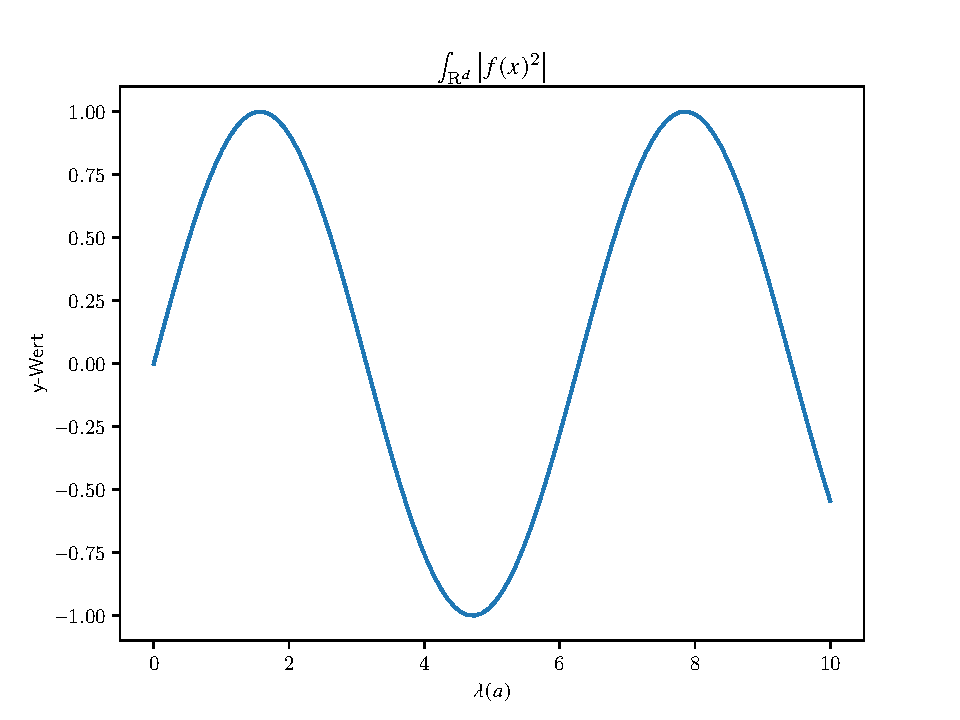
\includegraphics[width=0.5\textwidth]{figures/plot.pdf}
    \caption{Sine function}
    \label{fig:sinus}
\end{figure}



%%%%%%%%%%%%%%%%%%%%%
\newpage
\section{Basic Formalism}
\subsection{schrödinger equation}

Basic Definitions of schröfinger qe, light dyson series, and strong field s matrix

We want the time evolution of a quantum system in the presence of an external time dependent field in order to describe the strong field ionization later on.
The time evolution of a quantum system is given by the time dependent Schrödinger equation and a general hamiltonian
\begin{equation}
    i \hbar \frac{\partial}{\partial t} \ket{\Psi(t)} = \hat{H}(t) \ket{\Psi(t)}. \label{eq:schroedinger}
\end{equation}
The formal solution depends on the time dependence of the hamiltonian and the physical setting. 
In the following we assume \footnote{How? Later. No physical setting bzw no approximations yet. Its better to juistify it later but have a working formalism instead of the other way around.} (IMPORTANT) that $[\hat{H}(t), \hat{H}(t')] = 0$ so we assume some sort of quasi static approximation to the Hamiltons time evolution. 
The solution is then given by 
\begin{equation}
    \ket{\Psi(t)} = e^{-\frac{i}{\hbar} \int_{t_0}^{t} \hat{H}(t') dt'} \ket{\Psi(t=0)}
\end{equation}
Now its time so establish a physical setting. We have Hydrogen Atom with nucleus and electron described by time indepentent Hamilton $\hat{H}_0$. 
The external laser Field is descirbed by an time dependent part $\hat{V}(t)$. To describe the interaction of the atom with the laser field we use in the following the dipole approximation.




%%%%%%%%%%%%%%%%%%%%%
\newpage
\subsection{Light-Matter Interaction}
A light wave is defined by the Maxwell equations
\begin{equation*}
    \begin{aligned}
        \nabla \cdot \mathbf{E}(t) &= \rho \quad & \nabla \times \mathbf{E}(t) &= -\frac{\partial \mathbf{B}(t)}{\partial t} \\
        \nabla \cdot \mathbf{B}(t) &= 0 \quad & \nabla \times \mathbf{B}(t) &= \mathbf{J} + \frac{\partial \mathbf{E}(t)}{\partial t}
    \end{aligned}
\end{equation*}
The Maxwell equations are being solved by
\begin{equation*}
    \begin{aligned}
        \mathbf{E}(t) &= -\nabla \phi(t) - \frac{\partial \mathbf{A}(t)}{\partial t}\\
        \mathbf{B}(t) &= \nabla \times \mathbf{A}(t)
    \end{aligned}
\end{equation*}
For these solutions we introduced the vector potential $\mathbf{A}(t)$ and the scalar potential $\phi(t)$. 
These are not unique such that different choices can result in the same physical setting. In general
\begin{equation*}
    \begin{aligned}
        \mathbf{A}(t) &\to \mathbf{A}(t) + \nabla \chi(t) \\
        \phi(t) &\to \phi(t) - \frac{\partial}{\partial t} \chi(t)    
    \end{aligned}
\end{equation*}
also fulfill the Maxwell equations while $\chi(t)$ is an arbitrary smooth function. The arbitrariness of $\chi$ is known as gauge freedom and a direct consequence of the Maxwell equations.
Choosing a gauge (i.e., a specific $\chi$) is a matter of convenience and can be used to simplify the calculations as presented in the following.




\subsection{Dipole Approximation}
Very important approximation. Making it implies that
\begin{equation}
    \mathbf{A}(\mathbf{x}, t) \approx \mathbf{A}(t) \quad \text{and} \quad \mathbf{B} = \nabla \times \mathbf{A} \approx 0
\end{equation}
Therefore we can rewirte the time dependent part $\hat{V}$ of our Hamiltonian as
\begin{equation}
    \hat{V}(t) = -\hat{\mathbf{d}} \cdot \mathbf{E}(t)
\end{equation}
where $\hat{\mathbf{d}}$ is the dipole operator and $\mathbf{E}(t)$ is the electric field.




%%%%%%%%%%%%%%%%%%%
\newpage
\section{Strong Field Approximation}
%clear defintition of the strong field approximation, and the assumptions that are made.

For making the strong field approximation we first have to obtain a poitn where is its good to use. 
When we treat $\hat{V}(t)$ as the interaction term, we can write an exakt solution to \eqref{eq:schroedinger}
\begin{equation}
    \ket{\Psi(t)} = e^{-\frac{i}{\hbar} \int_{t_0}^{t} \hat{H}(t') dt'} \ket{\Psi(t=0)} + \int_{t_0}^{t} dt' e^{-\frac{i}{\hbar} \int_{t'}^{t} \hat{H}(t'') dt''} \hat{V}(t') e^{-\frac{i}{\hbar} \int_{t_0}^{t'} \hat{H}(t'') dt''} \ket{\Psi(t=0)}
\end{equation}




%%%%%%%%%%%%%%%%%%%%%
\newpage
\section{Strong Field Ionization}

Derivation of 

\begin{equation}
    \lim_{t \to \infty} \ket{\Psi(t)}  = -i \int d^3 p\, \ket{\mathbf{p}} \int_{-\infty}^{\infty} dt'\, e^{-\frac{i}{2}\int_{t'}^{\infty} [\mathbf{p}+\mathbf{A}(t')]^2 \, dt'} e^{i I_\mathrm{p} t'} \langle \mathbf{p} + \mathbf{A}(t') | \hat{\mathbf{d}} \cdot \mathbf{E}(t') | \Psi_0 \rangle
\end{equation}





%%%%%%%%%%%%%%%%%%%%
\newpage
\section{Multiphoton Ionization}

Different types of Ionization, tunneling Ionization, multiphoton